\documentclass[tikz]{standalone}

\usetikzlibrary{patterns}

\begin{document}
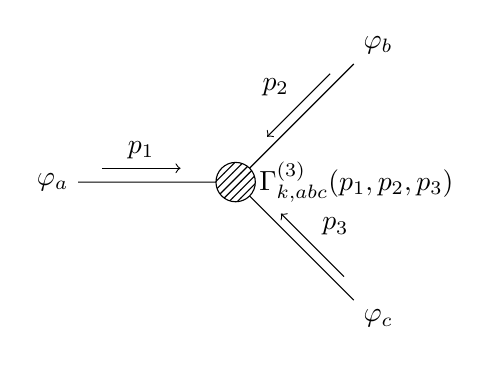
\begin{tikzpicture}
  \draw (-2,0) node[left] {$\varphi_a$} -- (0,0) -- (1.5,1.5) node[above right] {$\varphi_b$} (0,0) -- (1.5,-1.5) node[below right] {$\varphi_c$};
  \draw[->,yshift=5pt] (-1.7,0) -- (-0.7,0) node[midway,above] {$p_1$};
  \draw[<-,yshift=5pt] (0.4,0.4) -- (1.2,1.2) node[midway,above left] {$p_2$};
  \draw[<-,xshift=5pt] (0.4,-0.4) -- (1.2,-1.2) node[midway,above right] {$p_3$};
  \draw[fill=white,postaction={pattern=north east lines}] (0,0) circle (0.25) node[right=5pt] {$\Gamma_{k,abc}^{(3)}(p_1,p_2,p_3)$};
\end{tikzpicture}
\end{document}
